\section{Investigación}

Los algoritmos descritos a continuación son tomados del libro de \cite{needham2019graph}. 

\subsection{Strongly Connected Components}

El SCC hace referencia a un algoritmo que encuentra conjuntos de nodos conectados en grafos directos; donde cada nodo es alcanzable en ambas direcciones desde cualquier otro nodo del mismo conjunto. 

\begin{center}
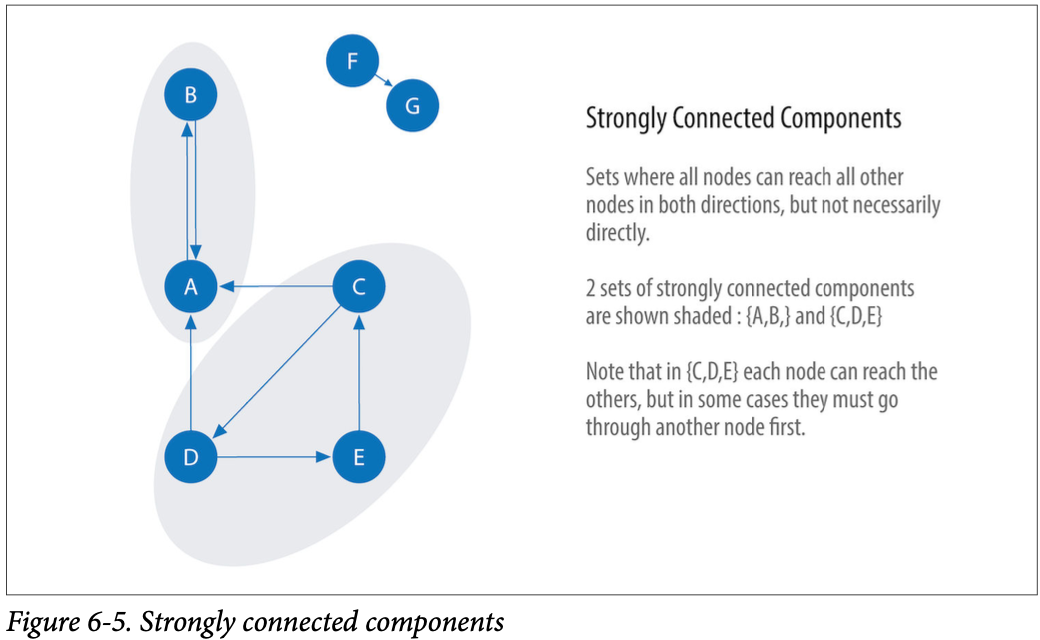
\includegraphics[scale=0.4]{Images/1-SCC.png}    
\end{center}

Características: 

\begin{itemize}
    \item No es necesario que los nodos sean vecinos, pero deben haber aristas entre todos los nodos del conjunto. 
    \item Descomponer un grafo directo en un algoritmo SCC es una aplicación de otro algoritmo: \textit{Depth First Search algorithm}.  
    \item Un componente fuertemente conectado tiene una utilidad directa o inclinación para encontrar comportamientos similares. 
\end{itemize}

\subsection{Betweenness Centrality}

Este es un algoritmo que tiene como propósito detectar la cantidad de influencia que un nodo tiene sobre un flujo de información o recursos de un grafo. Una analogía sería: un algoritmo que intenta encontrar nodos que sirvan como puentes de una parte del grafo hacia otra. 

Características: 

\begin{itemize}
    \item Este algoritmo primero calcula la trayectoria más corta (\textit{weighted}) entre cada par de nodos en un grafo conectado. Cada nodo recibe un puntaje, basado en el número de trayectorias que pasan a través del nodo. Entre más trayectorias cortas pase un nodo, más alto es su puntaje.
    \item Puentes y puntos de control 
    \begin{itemize}
        \item[Puente:] Puede ser un nodo o una relación. Se pueden identificar, ya que si si se remueve un punte, el grafo se convierte en un grafo disconexo. 
        \item[Pivote:] Un nodo es considerado pivote para otros dos nodos, si ese nodo está en la trayectoria más corta de esos dos nodos. Es decir: 
        \begin{center}
            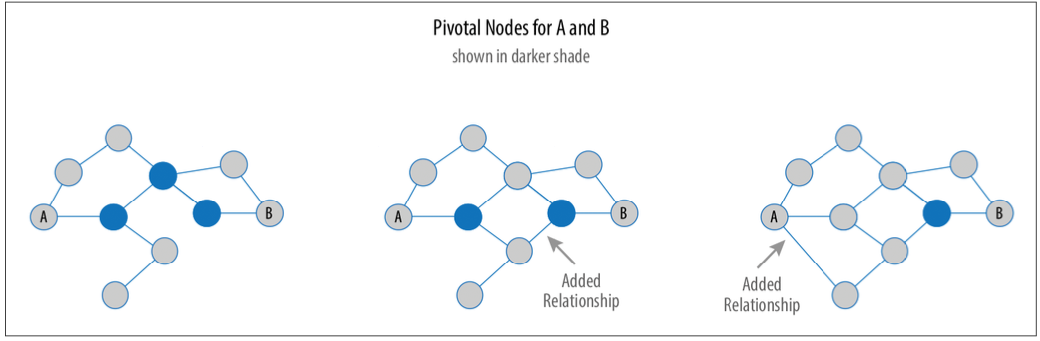
\includegraphics[scale=0.4]{Images/1-pivotal.png}
        \end{center}
    \end{itemize}
\end{itemize}
\subsubsection{¿Cómo se calcula el betweenness centrality?}

$$B(u)=\sum_{s\neq u\neq t}\frac{p(u)}{p}$$
En donde: 
\begin{enumerate}
    \item $u$ es un nodo. 
    \item $p$ es el número de trayectorias cortas entre los nodos $s$ y $t$.
    \item $p(u)$ es el número de trayectorias cortas entre los nodos $s$ y $t$ que pasan a través del nodo $u$. 
\end{enumerate}

\begin{center}
    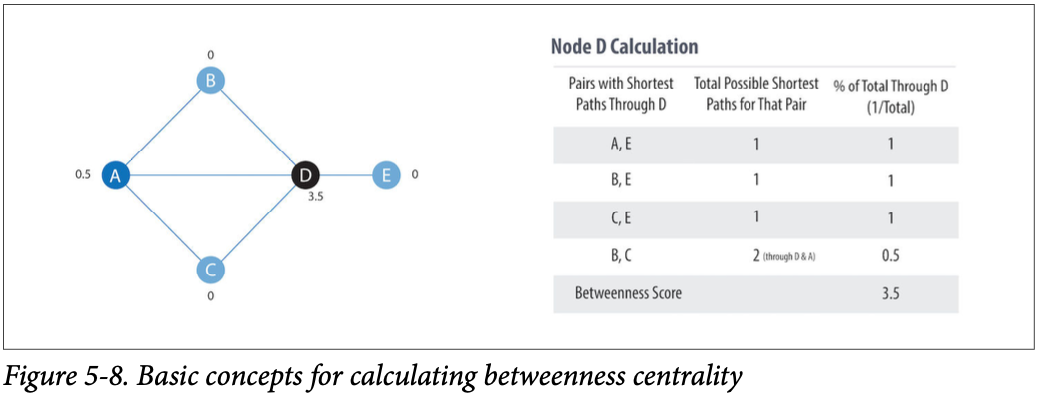
\includegraphics[scale=0.4]{Images/1-bc.png}
\end{center}

Un ejemplo: 

\begin{center}
    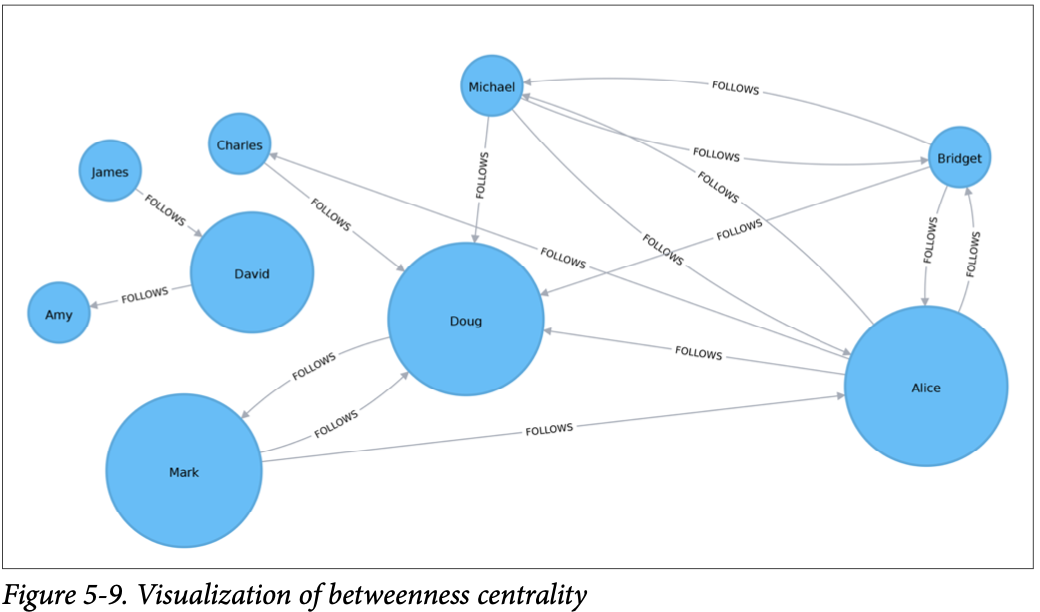
\includegraphics[scale=0.4]{Images/1-bc2.png}
\end{center}

\subsection{PageRank}
PageRank es el mejor algoritmo de centralidad conocido. El algoritmo mide la transitividad (o dirección) de la infuencia de los nodos. PageRank 
considera la influencia de los vecinos de un nodo y de sus vecinos. Por ejemplo, una analogía, una persona que tenga pocos amigos poderosos puede ser más influyente que alguien que tenga muchos amigos pero menos poderosos. 

\subsubsection{¿Cómo se calcula?}
Citando literalmente a \cite{needham2019graph}. «PageRank is defined in the original Google paper as follows: 
$$PR(U)=(1-d)+d\left(\frac{PR(T_1)}{C(T_1)}+\cdots +\frac{PR(T_n)}{C(T_n)}\right)$$
where: 

\begin{enumerate}
    \item  We assume that a page u has citations from pages $T_1$ to $T_n$.
    \item $d$ is a damping factor which is set between 0 and 1. It is usually set to 0.85. You can think of this as the probability that a user will continue clicking. This helps minimize rank sink, explained in the next section.
    \item $1-d$ is the probability that a node is reached directly without following any rela‐ tionships.
    \item $C(T_n)$ is defined as the out-degree of a node $T$.»
\end{enumerate}
\begin{center}
    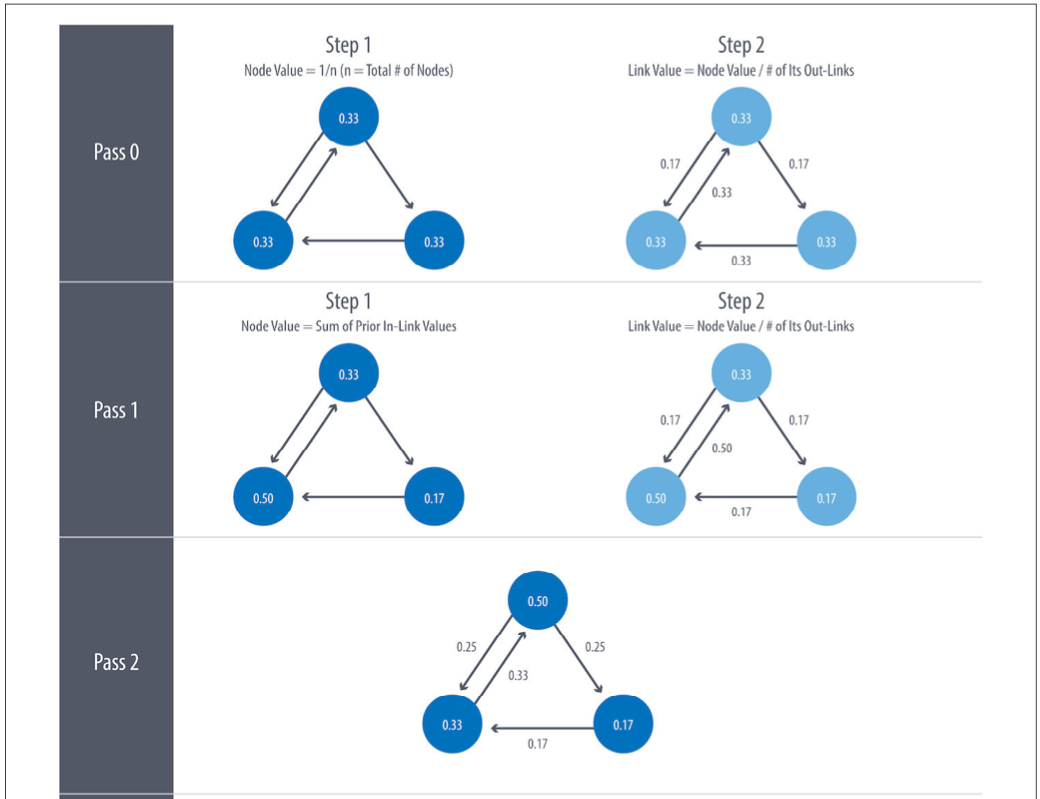
\includegraphics[scale=0.35]{Images/1-pr1.png}
    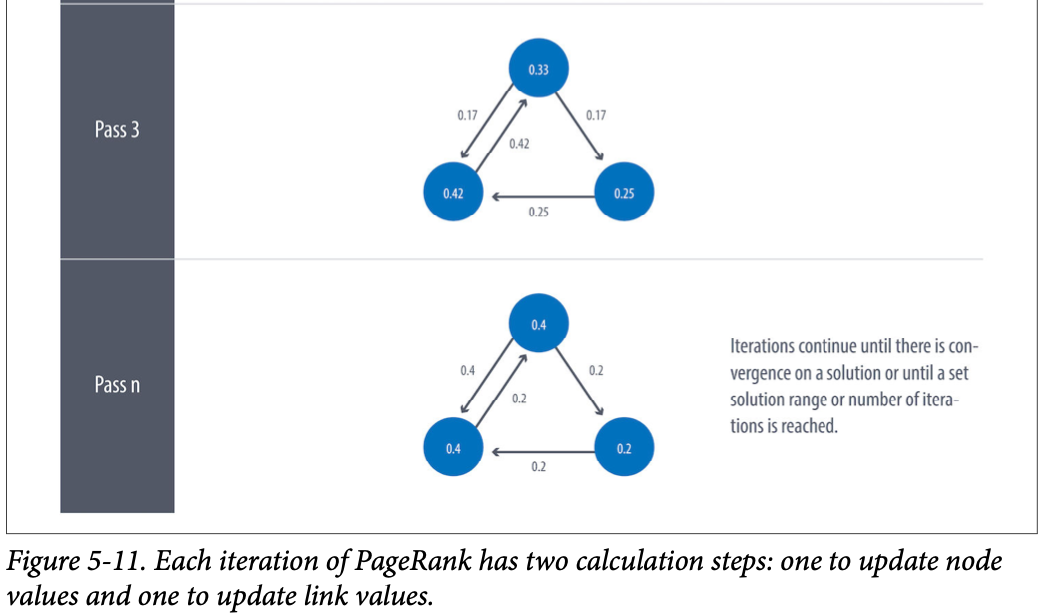
\includegraphics[scale=0.35]{Images/1-pr2.png}
\end{center}